We report results across 15 two-agent backbone$\times$domain$\times$topology configurations. The central question: in two-agent solver-checker systems, does perturbation sensitivity predict pruning safety?

\subsection{Impact Gradient}
\label{sec:impact_gradient}

For Qwen under fixed-turn topologies (Figure~\ref{fig:impact}), the impact gradient is inversely related to information content: \textsc{acknowledgment} (mean similarity $= 0.352$, $n = 450$), \textsc{information\_provision} ($0.410$, $n = 177$), \textsc{verification} ($0.616$, $n = 110$), \textsc{reasoning\_guidance} ($0.778$, $n = 158$). Informationally sparse acknowledgments are those whose removal is most disruptive.

\begin{figure}[t]
\centering
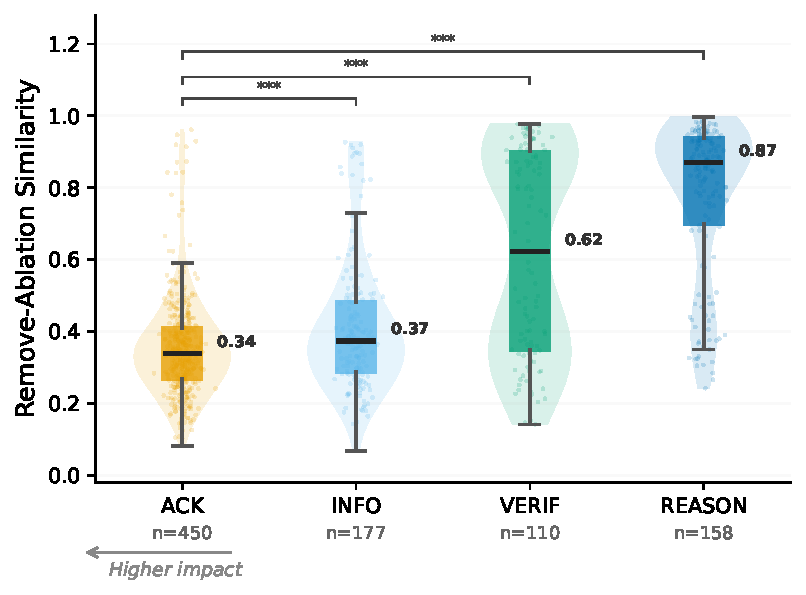
\includegraphics[width=\columnwidth]{figures/fig_impact.pdf}
\caption{Remove-ablation similarity by function type (Qwen2.5-7B, round-robin, $n = 895$). Lower = greater disruption. Acknowledgments (median $= 0.34$) are most impactful despite least information content.}
\label{fig:impact}
\end{figure}

\paragraph{Pruning evidence.} Removing a single acknowledgment is associated with high disruption (similarity $< 0.5$) in 91\% of cases vs.\ 19\% for reasoning guidance. The neutralize ablation produces the \emph{opposite} gradient: neutralized information provision is associated with maximal disruption ($0.047$) while neutralized acknowledgments are associated with only moderate disruption ($0.153$; Appendix~\ref{app:neutralize}). This double dissociation confirms acknowledgment impact stems from structural presence, not content. Robustness: placeholder choice $\rho = 0.73$; non-ack $\rho{=}0.90$; four similarity metrics $\rho > 0.91$ (Appendix~\ref{app:metric-robustness}); RR/SEQ consistent, selector breaks down.

\paragraph{Taxonomy-independent information measures.} Independent of taxonomic labels, acknowledgments are quantifiably information-sparse: Qwen acks have 5.7\% bigram novelty (vs.\ 74.9\% for reasoning guidance), median 4 tokens (vs.\ 117), and Jaccard overlap 0.69. Llama acks are longer (mean 59.8 tokens, 65.6\% bigram novelty) but exhibit 0\% error correction yet 14.3\% error injection---a one-directional error channel (Appendix~\ref{app:info_theory}).

\subsection{E2E Communication Pruning}
\label{sec:e2e_pruning}

The individual perturbation results above suggest acknowledgments should be critical to preserve. The aggregate pruning tests below reveal the opposite---a dissociation we analyze in Section~\ref{sec:discussion}.
We compare four strategies: \textbf{Baseline}, \textbf{Ack-only} (remove acknowledgments), \textbf{Function-Guided (FG)} (remove lowest-impact function type), and \textbf{Random} (same count as ack-only, 10 seeds).

\paragraph{Main results.} Despite their individual disruptive impact, acknowledgments can be safely pruned in aggregate (Table~\ref{tab:online_pruning}, Figure~\ref{fig:forest}). Both backbones show non-inferiority at $\delta = -3$\,pp ($p < 0.001$). Ten-seed Qwen oracle: $\Delta = +0.40 \pm 1.02$\,pp (95\% CI $[-0.33, +1.13]$\,pp; TOST $p = 0.048$ at $\pm 1$\,pp; 56.0\% suppression). Ten-seed Llama oracle: $\Delta = +2.1 \pm 2.4$\,pp (95\% CI $[+0.4, +3.8]$\,pp; 9/10 positive). The positive direction reflects a one-directional error channel (0/1{,}483 corrections but non-zero injection; Fisher $p = 0.004$).
Non-inferiority ($p < 0.001$) provides the primary safety evidence; TOST provides supplementary equivalence precision (Qwen oracle $p = 0.048$, marginal; interpret alongside CI).

Message-level suppression (36--56\%) translates to lower token-level savings (${\sim}10\%$ Qwen, ${\sim}28\%$ Llama; Appendix~\ref{app:efficiency}) because acknowledgments are shorter than substantive messages; the primary efficiency gain is inference-call elimination, not token reduction.

Heuristic detectors confirm deployment feasibility: Qwen 10~runs $\Delta = -0.05 \pm 0.99$\,pp (TOST $p = 0.007$ at $\pm 1$\,pp). Llama 5~seeds $\Delta = +2.20 \pm 1.44$\,pp (95\% CI $[+0.41, +3.99]$\,pp; non-inferiority $p < 0.001$): pruning is not merely non-inferior but suggestive of a small beneficial effect, though the interval width and limited seed count~(5) preclude a strong improvement claim. The heuristic over-suppresses (${\sim}75\%$ vs.\ ${\sim}37\%$ oracle rate), yet the positive direction suggests over-suppressed messages are predominantly redundant.
Qwen StrategyQA (5~seeds) yields $\Delta = +0.70 \pm 0.91$\,pp (95\% CI $[-0.43, +1.83]$), consistent with non-inferiority (p < 0.001 at $\delta = -3$\,pp).
The Llama StrategyQA heuristic (8~seeds) yields $\Delta = +2.81 \pm 3.94$\,pp (95\% CI $[-0.49, +6.11]$), directionally positive but with high seed-level variance; non-inferiority holds (CI lower bound $> -3$\,pp) with suppress rate stable across seeds (49--52\%).
Under stochastic decoding ($t{=}0.7$), pruning safety is backbone-dependent: Qwen oracle ($\Delta = +0.30 \pm 1.80$\,pp, 10 seeds; TOST $p < 0.001$ at $\delta = -3$\,pp) remains safe, while Llama shows marginal degradation (pooled $\Delta = -2.2$\,pp, Fisher $p = 0.29$, NS; Appendix~\ref{app:temp-robustness}).

\begin{table}[t]
\centering
\caption{Online suppression pruning accuracy (\%, $N$ tasks, McNemar exact $p$). All rows use online suppression (messages intercepted during live agent interaction; cf.\ remove-one ablation in \S\ref{sec:perturbation}, offline replay in Appendix~\ref{app:statistical}). \emph{Oracle}: GPT-4o 5-class ack-only. \emph{Heuristic}: annotation-free rules (F1 $= 0.845$/$0.805$). Multi-seed rows report $\Delta \pm \text{SD}$ (pp). Supp.\ = messages suppressed.\protect\footnotemark}
\label{tab:online_pruning}
\small
\begin{tabular}{lccccr}
\toprule
\textbf{Setting} & $N$ & \textbf{Baseline} & \textbf{Pruned} & $p$ & \textbf{Supp.} \\
\midrule
\multicolumn{6}{l}{\textit{Oracle (GPT-4o 5-class, ack-only)}} \\
\rowcolor{blue!4}
Llama / GSM8K & 500 & 82.2 & 81.6 ($-0.6$) & .710 & 36.6\% \\
\rowcolor{blue!4}
Qwen / GSM8K & 500 & 88.8 & 89.6 ($+0.8$) & .340 & 56.3\% \\
\rowcolor{blue!4}
Llama / GSM8K ($t{=}0.7$) & 500 & 82.2 & 79.2 ($-3.0$) & .150 & 28.0\% \\
\rowcolor{blue!4}
Qwen / GSM8K ($t{=}0.7$) & 500 & 87.4 & 88.0 ($+0.6$) & .710 & 53.1\% \\
\rowcolor{blue!4}
Qwen / GSM8K ($t{=}0.7$, 10 seeds) & 10${\times}$200 & \multicolumn{2}{c}{$\Delta = +0.30 \pm 1.80$\,pp} & ${<}.001$\textsuperscript{$\ddagger$} & 39.2\% \\
\rowcolor{blue!4}
Qwen / StratQA & 500 & 73.2 & 73.4 ($+0.2$) & 1.000 & 65.6\% \\
\rowcolor{blue!4}
Llama / StratQA\textsuperscript{$\S$} & 238 & 68.9 & 73.9 ($+5.0$) & .180 & 21.5\% \\
\rowcolor{blue!4}
Qwen / ARC & \arcN{} & \arcQwenBaseline{} & \arcQwenPruned{} ($\arcQwenDelta{}$) & \arcQwenPvalue{} & \arcQwenSupp{}\% \\
\rowcolor{blue!4}
Qwen / GSM8K (10 seeds) & 10${\times}$200 & \multicolumn{2}{c}{$\Delta = +0.40 \pm 1.02$\,pp} & .048\textsuperscript{$\dagger$} & 56.0\% \\
\rowcolor{blue!4}
Llama / GSM8K (10 seeds) & 10${\times}$200\textsuperscript{$\P$} & \multicolumn{2}{c}{$\Delta = +2.1 \pm 2.4$\,pp} & ${<}.001$\textsuperscript{$\ddagger$} & 36.5\% \\
\midrule
\multicolumn{6}{l}{\textit{Token-matched random (online control)}} \\
Qwen / GSM8K & 500 & 88.8 & 89.6 ($+0.8$) & .340 & 9.9\% \\
\midrule
\multicolumn{6}{l}{\textit{Heuristic (annotation-free, exploratory)}} \\
Llama / GSM8K (5 seeds) & 5${\times}$200 & \multicolumn{2}{c}{$\Delta = +2.20 \pm 1.44$\,pp} & ${<}.001$\textsuperscript{$\ddagger$} & 74.9\% \\
Qwen / GSM8K (10 runs) & 10${\times}$200 & \multicolumn{2}{c}{$\Delta = -0.05 \pm 0.99$\,pp} & .880 & 41.8\% \\
Qwen / StratQA (5 seeds) & 5${\times}$200 & \multicolumn{2}{c}{$\Delta = +0.70 \pm 0.91$\,pp} & ${<}.001$\textsuperscript{$\ddagger$} & 56.9\% \\
Llama / StratQA (8 seeds) & 8${\times}$200 & \multicolumn{2}{c}{$\Delta = +2.81 \pm 3.94$\,pp} & .002\textsuperscript{$\ddagger$} & 50.3\% \\
Qwen / GSM8K ($t{=}0.7$) & 500 & 88.6 & 88.0 ($-0.6$) & .730 & 37.3\% \\
Llama / GSM8K ($t{=}0.7$) & 500 & 81.2 & 77.8 ($-3.4$) & .100 & 59.3\% \\
\midrule
\multicolumn{6}{l}{\textit{Length-only baseline (char $< 30$)}} \\
Llama / GSM8K (5 seeds) & 5${\times}$200 & \multicolumn{2}{c}{$\Delta = -0.10 \pm 1.29$\,pp} & — & 0.8\% \\
Qwen / GSM8K (3 seeds) & 3${\times}$200 & \multicolumn{2}{c}{$\Delta = +0.50 \pm 1.50$\,pp} & — & 42.2\% \\
\bottomrule
\end{tabular}
\end{table}
\footnotetext{$^\dagger$TOST $\pm 1$\,pp (marginal). $^\ddagger$Non-inferiority $\delta = -3$\,pp. $^\S$Context overflow. $^\P$$N{=}1{,}939$ after filtering (${\sim}3\%$ loss).}

\begin{figure}[t]
\centering
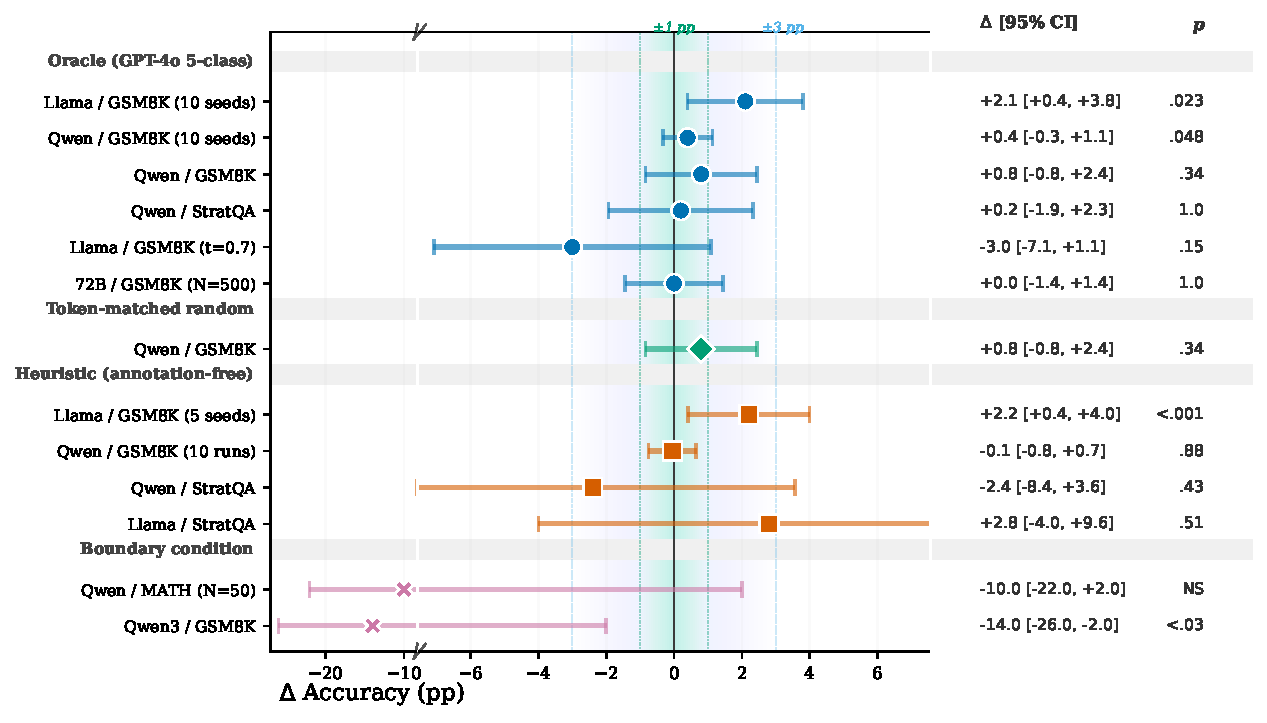
\includegraphics[width=\columnwidth]{figures/fig_forest.pdf}
\caption{Forest plot of pruning accuracy deltas ($\Delta$\,pp) with 95\% CIs. Green/blue bands: $\pm 1$\,pp TOST / $\pm 3$\,pp practical margins. Oracle and heuristic multi-seed results cluster near zero for Qwen; Llama heuristic shows a positive trend. Boundary conditions (MATH, Qwen3) show degradation.}
\label{fig:forest}
\end{figure}

In exploratory offline comparison ($N{=}100$, Qwen), FG pruning showed a substantial accuracy gap relative to ack-only ($-5.0$\,pp vs.\ $+1.0$\,pp, $p = 0.031$, exploratory), indicating aggregate safety is ack-specific. Online FG is confounded by cascading suppression (${\sim}90\%$ removal). Robust to 20\% label noise (Appendix~\ref{app:statistical}).

\paragraph{Token-matched random baseline.} Online random ($N{=}500$, Qwen) matches ack-only ($\Delta = +0.8$\,pp, NS), but ack-only suppresses $5.7\times$ more messages (56.3\% vs.\ 9.9\%) without per-task calibration. Per-task paired comparison confirms near-identical outcomes: only 4/500 tasks differ between strategies (McNemar $p = 1.0$; ack risk of correct$\to$wrong flip: 0.7\%, identical to random), demonstrating that acknowledgments are genuinely information-free---removing $5.7\times$ more of them produces zero additional harm. For Llama, ack-only significantly outperforms matched-count random removal (83\% vs.\ 73.2\%), ruling out conversation shortening as the explanation.

\paragraph{Length-only baseline.} A character-length filter ($< 30$ chars) yields backbone-divergent results (Table~\ref{tab:online_pruning}). For Qwen, it matches composite heuristic performance ($\Delta = +0.50 \pm 1.50$\,pp, 3~seeds; $p = 0.59$), confirming length as the primary discriminative axis. For Llama, the filter is near-vacuous (0.8\% suppression) while the composite heuristic suppresses ${\sim}75\%$, confirming that keyword and repetition rules are essential (\S\ref{sec:three_modes}).

\paragraph{Scale and heuristic detectors.} Pruning safety is directionally consistent across Qwen2.5 scales (7B/14B/72B; Appendix~\ref{app:scaling}). Full-scale 72B oracle ($N{=}\qwenSevenTwoBN{}$, single seed): $\Delta = \qwenSevenTwoBDelta{}$\,pp ($p = \qwenSevenTwoBPvalue{}$). Heuristic detectors achieve F1 $= 0.845$ (Qwen) and $0.805$ (Llama) without LLM annotation.

\subsection{Backbone Communication Typology}
\label{sec:three_modes}

Mixed-effects models ($N = 2{,}294$) reveal three topology-stable communication profiles: \textbf{function-organized} (Qwen), \textbf{position-organized} (Gemma; exploratory---$\kappa = 0.35$, below threshold, $< 5\%$ acks on GSM8K), and \textbf{undifferentiated} (Llama). Backbone $\times$ function\_type interaction is highly significant ($p < 10^{-41}$), stable across topologies (three-way $p = 0.963$). Selector topology attenuates Qwen's function-organization and slightly amplifies Llama's (Appendix~\ref{app:statistical}).

\subsection{Cross-Domain Consistency}
\label{sec:cross_domain}

Backbone dominates communication patterns (Cram\'{e}r's $V = 0.45$~\cite{cramer_1946} vs.\ $0.18$ for domain; Table~\ref{app:tab:me_results}). The $2 \times \numDomainCells{}$ cross-backbone$\times$cross-domain oracle matrix yields all cells NS (Table~\ref{tab:online_pruning}), attributing any heuristic StratQA residual to detector error (F1 $= 0.21$); MATH defines a domain boundary (\S\ref{sec:boundary}).

\paragraph{ARC-Challenge.} Oracle pruning on ARC-Challenge (Qwen, online re-generation; $N{=}\arcN{}$, $\Delta = \arcQwenDelta{}$\,pp, $p = \arcQwenPvalue{}$, \arcQwenSupp{}\% suppression) extends cross-domain validation to a third reasoning domain. Offline simulation on Llama is directionally consistent with the online pattern: baseline $\arcLlamaBaseline{}\%$ $\to$ pruned $\arcLlamaPruned{}\%$ ($N{=}\arcLlamaN{}$, $\Delta = \arcLlamaDelta{}$\,pp, $p = \arcLlamaPvalue{}$, $\arcLlamaSupp{}\%$ suppression), strengthening dual-backbone evidence on ARC despite the methodological difference (simulate mode re-extracts answers from pruned traces rather than re-generating responses).

\subsection{Boundary Conditions}
\label{sec:boundary}

Three boundary conditions define pruning limits. (1)~\emph{Domain mismatch}: MATH yields $\Delta = -2.0$\,pp (NS, $N{=}200$, 102 valid; Appendix~\ref{app:math}), with acks qualitatively different from GSM8K (16.6 tokens, 33\% bigram novelty vs.\ 5.6 tokens, 0\%). (2)~\emph{Heuristic non-transferability}: Qwen3-8B's ack format (25--59 chars) bypasses the v1 heuristic; a wider char$<$80 threshold reaches $\Delta = -14$\,pp ($p < .03$), confounded with non-ack suppression (Appendix~\ref{app:qwen3_comparison}). (3)~\emph{Online cross-domain}: Qwen StratQA heuristic (5~seeds) yields $\Delta = +0.70$\,pp (NS), consistent with non-inferiority; the earlier single-seed estimate ($-2.4$\,pp, $N{=}250$) is superseded by the more reliable 5-seed replication ($N{=}200 \times 5$; oracle $+0.2$\,pp). We recommend empirical screening ($N \geq 200$, ${\geq}\,80\%$ power for ${\geq}\,5$\,pp effects) before deployment.
